\subsection{Identification of PID parameters using Relay Feedback Technique}
Relay feedback auto-tuning method developed by Astrom and Huggland is
one of the simplest and most popular auto-tuning technique for process
control applications\cite{karl84}. In this method, a simple
experimental test is used to determine ultimate gain and ultimate
period. 

\begin{figure}
\hspace{-0.2in}
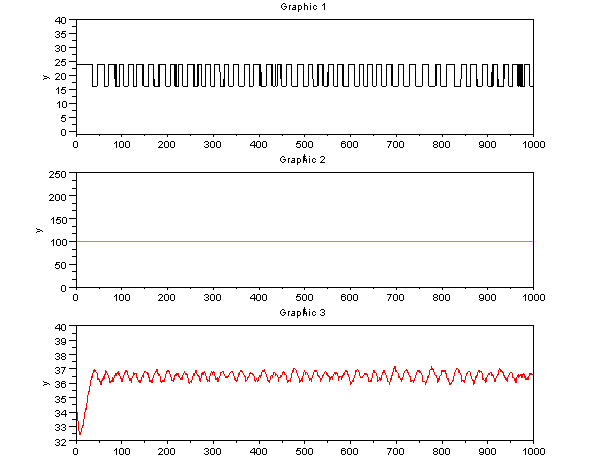
\includegraphics[width=1.2\linewidth]{figures/relay.png}
\caption{Relay feedback implementation: heater duty, fan speed,
  temperature} 
\label{relayresp}
\end{figure}

\begin{figure}
\centering
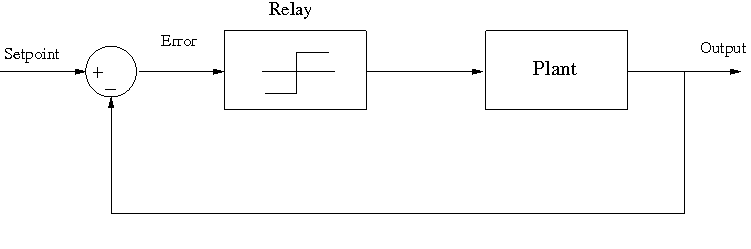
\includegraphics[width=\linewidth]{figures/relay1.png}
\caption{Conventional relay feedback system}
\label{relaysys}
\end{figure}

A feedback controller is temporarily repalced by an On-Off controller (or a relay) as shown in the Figure \ref{relaysys}. When the control loop is closed, the control variable exhibits a sustained oscillations which is a property of On-Off controller.

Relay feedback method has been implemented on Single board heater system using virtual labs.


From the Figure \ref{relayresp}, we can observe the sustained
oscillations in temperature. 
Using the expressions derived by \cite{karl84}, the following
parameters are obtained:
The Ultimate period Pu = 25 seconds.
The Ultimate gain Kc = 5.66.  The                    
PID parameters are then calculated from Ziegler-Nichols controller
settings shown in Table \ref{2ndmtd}. 
\begin{table}
\begin{center}
\renewcommand{\arraystretch}{1.5}
\begin{tabular}{|c|r|r|r|}\hline
Type of
controller & $K_{c}$ & $\tau_i$ & $\tau_d$ \\ \hline
$P$ & $0.5K_{cu}$ & $\infty$ & 0 \\ \hline
$PI$ & $0.45K_{cu}$ & $ 0.8334P_{u}$ & 0 \\\hline
$PID$ & $0.6K_{cu}$ & $0.5P_{u}$ & $0.125P_{u}$ \\ \hline
\end{tabular}
\caption{Ziegler-Nichols Controller Settings based on the Continous Cycling Method}
\label{2ndmtd}
\end{center}
\end{table}%
The PID parameters are obtained as
$K_{c}$ = 3.3939394,
$\tau_i$ = 12.5, and 
$\tau_d$ = 3.125.


           
